%-------------------------------------------------------------------------------
\chapter{Design Space Exploration Methodology}
\labelchapter{ch.dse}
%-------------------------------------------------------------------------------

%%%%%%%%%%%%%%%%%%%%%%%%%%%%%%%%%%%%%%%%%%%%%%%%%%%%%%%%%%%%%%%%%%%%%%%%%%%%%%%%
%%%%%%%%%%%%%%%%%%%%%%%%%%%%%%%%%%%%%%%%%%%%%%%%%%%%%%%%%%%%%%%%%%%%%%%%%%%%%%%%

\lettrine[lines=2]{A}{fter} defining the interest of relevant metrics and accurate estimators for hardware development processes, we focus on their usage for \myLongAc{DSE}{Design Space Exploration}.
This chapter outlines the specificities of \myLongAcs{HCL}{Hardware Construction Language} that can be used for efficient \myAc{DSE}, before proposing a methodology for \myAc{HCL}-based \myAc{DSE}.
This methodology is based on high level programming features such as \myLongAc{OOP}{Object-Oriented Programming} or functional programming, which enable more expressivity for the developers.
We also exhibit the limitations of this approach and discuss various solutions to improve the proposed methodology.

\vspace*{\fill}
\minitoc 
\mtcskip 

\newpage
%%%%%%%%%%%%%%%%%%%%%%%%%%%%%%%%%%%%%%%%%%%%%%%%%%%%%%%%%%%%%%%%%%%%%%%%%%%%%%%%

\section[Defining DSE in a HCL context]{Defining Design Space Exploration using Hardware Construction Languages}
\label{ch.dse:sec.definition}

    This section aims at defining how \myLongAcs{HCL}{Hardware Construction Language} specificities can be leveraged for efficient \myLongAc{DSE}{Design Space Exploration}, in contrast to other \myAc{DSE} methodologies based on various paradigms.

    The \myAc{HCL} paradigm enables to describe hardware circuit generators instead of hardware circuits, allowing to fully control generated hardware at \myLongAc{RTL}{Register-Transfer Level}.
    Doing so, we can define \myAc{DSE} methodologies which leverage the developers expertise to reduce the amount of implementations to explore, as some of them can easily be pruned considering prior knowledge on both algorithm and target.
    Moreover, high level features such as \myLongAc{OOP}{Object-Oriented Programming} or functional programming can be used to expose variations, exposing more complex implementation options --- such as the definition of various computation units using functions as module parameters --- when compared to standard \myAc{DSE} flows, such as \myLongAc{HLS}{High Level Synthesis} methodologies.

    \subsection{Meta Design and Meta Exploration}
    \label{ch.dse:sec.definition:ssec.meta}
        In order to propose an efficient \myAc{HCL}-based \myAc{DSE} methodology, we start by defining two main concepts: {\bf meta design} and {\bf meta exploration}.

        {\bf Meta design} is defined as the process of building an explorable design generator based on a prior analysis of both algorithm and target (Fig. \ref{ch.dse:sec.definition:ssec.meta:fig.meta-design}).
        Leveraging this analysis, a developer can define relevant implementation variations --- meaning that each possible implementation results from a choice from the user --- and expose them at top level, directly in the module constructor.
        Doing so, the exploration process no more relies on tool inferences to generate such variations --- \eg as it is the case with \myAc{HLS} methodologies --- but on controlled variations of the generators, resulting in a more meaningful design space to be explored.
        Moreover, using such methodologies enable a more intelligible approach of the exploration, as the implementation options are directly defined by users, enabling a better apprehension of their impacts on the generated design.
        
        \begin{figure}[h!]
            \centering
            
\includegraphics[width=0.9\textwidth]{Figures/Methodology-metadesign}
            \caption{Meta design methodology}
            \label{ch.dse:sec.definition:ssec.meta:fig.meta-design}
        \end{figure}

\clearpage
        We then define {\bf meta exploration} (Fig. \ref{ch.dse:sec.definition:ssec.meta:fig.meta-exploration}) as a process exploiting a design generator --- that was built using {\bf meta design} --- to explore its implementation variations, thus defining a \myAc{HCL}-based \myAc{DSE} methodology.
        In order to provide efficient exploration processes, this methodology allows the users to define custom strategies --- after defining the design space --- leveraging their expertise to guide the flow.
        In the next sections, we will consider a strategy to be composed of various metrics to be estimated (with respect to the considerations introduced in Chapter \ref{ch.estimators}), as well as the different steps to browse the design space (see Section \ref{ch.dse:sec.functional}).
        \begin{figure}[h!]
            \centering
            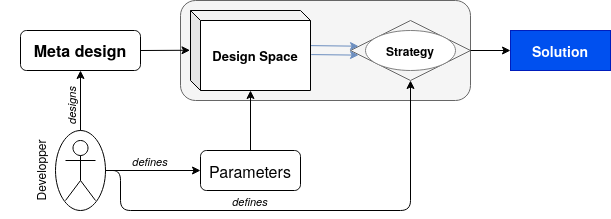
\includegraphics[width=1.0\textwidth]{Figures/Methodology-metaexploration}
            \caption{Meta exploration methodology}
            \label{ch.dse:sec.definition:ssec.meta:fig.meta-exploration}
        \end{figure}

    \subsection{Implementation Knobs and Parameters}
    \label{ch.dse:sec.definition:ssec.knobs}

        As seen in Section \ref{ch.state:sec.space:ssec.mixing}, \myAc{HLS} and \myLongAcs{DSL}{Domain Specific Language} based \myAc{DSE} methodologies are based on {\bf knobs} --- \ie implementation options --- which can be of three kinds: local attributes (as pragmas), global synthesis options and \myLongAcs{FU}{Functional Unit} options \cite{schafer_high-level_2020}.

        The exploration knobs are used by \myAc{DSE} tools to generate implementation variations, resulting in an explorable space of equivalent implementations of a same algorithm.
        It is thus comparable to the parameters of {\bf meta design} based circuit generators as defined in Section \ref{ch.dse:sec.definition:ssec.meta}.

        However, the high level parameters exposed by the {\bf meta design} methodology cannot express global synthesis options as it is done with knobs, and such variations must thus be considered in the {\bf meta exploration} strategy, in order to offer comparable features.
        Nevertheless, both local attributes and \myAc{FU} options can be leveraged using design generator parameters, and will then be used in this work to define explorable design spaces.

%%%%%%%%%%%%%%%%%%%%%%%%%%%%%%%%%%%%%%%%%%%%%%%%%%%%%%%%%%%%%%%%%%%%%%%%%%%%%%%%%

\section{Building Explorable Architectures}
\label{ch.dse:sec.explorable}
    As defined in the previous section, the first step to define our \myAc{HCL}-based \myAc{DSE} methodology is to build an efficient {\bf meta design} method.

    \subsection{Designing Explorable Hardware Generators}
    \label{ch.dse:sec.explorable:ssec.generators}
        To design explorable hardware generators, one should begin by analysing both the algorithm and the target to exhibit meaningful implementation variations.
        It should result in a design space of relevant architectures to be explored, while leveraging the users expertise to expose both specific and non specific parameters.

        For example, the \myLongAc{IO}{Input/Output} bandwidth is a non specific parameter, as it will have a significant impact on most of circuits, while the potential of parallelism or the number of a particular \myAc{FU} in a given architecture is application specific, as it will not have the same impact nor the same definition, depending on the targeted algorithm.
        The user expertise is thus required to produce a good analysis, and is primordial for this whole methodology to produce meaningful results.

        After defining the exploration parameters, one needs to exhibit the possible values for each of them, in order to build the design space --- \ie a set of parameters which will be used in elaboration to give a particular implementation.
        For each parameter, users thus need to define a set of possible values, and each set is then considered in a {\bf cartesian product} to build the resulting design space.

        In order to integrate the {\bf meta design} methodology in an \myLongAc{HCF}{Hardware Construction Framework}, we propose to expose both parameters and their values at circuit top levels, in order to build intelligible flows and allow easy evolutions of the exploration processes.

        \begin{figure}[h!]
            \begin{lstlisting}[xleftmargin=0mm,
                               caption={Exposing the dot product design space},
                               label={ch.dse:sec.explorable:ssec.generators:list.dotproduct}]
class DotProduct(
  @linear(6, 12)    dynamic: Int,
  @linear(6, 12)    precision: Int,
  @enum(16)         nElem: Int,
  @linear(0, 4)     parallelism: Int
) extends Module with Explorable\end{lstlisting}
        \end{figure}

\clearpage
        In Listing \ref{ch.dse:sec.explorable:ssec.generators:list.dotproduct}, we use \chisel{} constructors to expose the design space of a {\bf dot product} design, computing the dot product of two vectors $a_n$ and $b_n$.\footnote{Given $a_n = (a_0, ..., a_{n-1})$ and $b_n = (b_0, ..., b_{n-1})$, we compute $c = \sum_{i = 0}^{n-1} a_i * b_i$.}
        
        We define four different parameters, namely the element dynamic and precision in bits (as the circuit only consider fixed point elements), the number of elements in each vector and the level of parallelism.

        For each parameter, we only consider integer values for simplicity purpose, and define different set generators in Figure \ref{ch.dse:sec.explorable:ssec.generators:fig.annotations}.
        \begin{figure}[ht!]
            \centering
            \begin{itemize}
                \item \lstinline{@byX(x, y)} $\Leftrightarrow$\hspace*{\fill}$p \in [\![x, y]\!] \land p \equiv 0 \pmod X$
                \item \lstinline{@linear(x, y)}\footnotemark$\Leftrightarrow$\hspace*{\fill}$p \in [\![x, y]\!]$
                \item \lstinline{@enum(x0, ..., xn)} $\Leftrightarrow$ \hspace*{\fill} $p \in \{x_0, ..., x_n\} \land \forall i \in [\![0, n]\!], x_i \in \mathbb{N}$
                \item \lstinline{@powX(x, y)} $\Leftrightarrow$\hspace*{\fill}$p \in \mathbb{N}/p = X^z \land z \in [\![x, y]\!]$
                \item \lstinline{@pow2(x, y)} $\Leftrightarrow$\hspace*{\fill}$p \in \mathbb{N}/p = 2^z \land z \in [\![x, y]\!]$
            \end{itemize}
            \caption{Annotation based parameter generation}
            \label{ch.dse:sec.explorable:ssec.generators:fig.annotations}
        \end{figure}
        \footnotetext[\thefootnote]{Equivalent to \lstinline{@by1(x, y)}.}

        We use the \scala{} annotation system to directly annotate the constructor parameters with value generators, thus embedding both parameters and their values in the top level module --- \ie the entry point of the \chisel{} flow.

        For the {\bf dot product} algorithm, we thus build a $7 \times 7 \times 1 \times 5 = 245$ wide design space to be explored, using the cartesian product of each set of possible values: both {\it dynamic} and {\it precision} can each take $|[\![6, 12]\!]| = 7$ different values, while {\it parallelism} can take 5, and {\it nElem} is fixed.

    \subsection{Impact of the Implementation Parameters}
    \label{ch.dse:sec.explorable:ssec.impact}
        This approach allows to define the design space in an easy way by integrating it directly in the top level module, through its constructor.

        However, leveraging the user expertise is not only about defining meaningful parameters and their values for the exploration, but also about bringing information about how the parameter variations may impact the exploration processes.
        For example, in the {\bf dot product} implementations, we can state that the three first parameters --- namely {\it dynamic}, {\it precision} and {\it nElem} --- impact the algorithm \myLongAc{QoS}{Quality of Service}, while the fourth one --- {\it parallelism} --- does not, as it only impacts the latency of the generated circuit.

        In order to improve this first approach with respect to this observation, we thus need a way to define if a particular parameter variations has an impact on a given metric.
        With such feature, a given exploration step that considers only the \myAc{QoS} of the designs will not consider the fourth dimension of the {\bf dot product} generator, as every variation of the fourth parameter in the design space is to be considered equivalent with respect to the \myAc{QoS}.
        This enables to reduce the design space, dividing the number of implementations to explore by a factor 5 --- the cardinality of the {\it parallelism} set of values --- for an exhaustive exploration process.

    \subsection[Exposing an Expertised Based Design Space]{Exposing an Expertise Based Design Space for Exploration}
    \label{ch.dse:sec.explorable:ssec.space}

        In order to enhance design space with informations on how chosen parameters impact given metrics, we add yet another annotation system to module constructors, in a way similar to the one introduced in Section \ref{ch.dse:sec.explorable:ssec.generators}.
        We thus add a \lstinline{@qualityOfService} annotation, which bears the information that the annotated parameter does impact the \myAc{QoS} metric.

            \begin{figure}[h!]
                \vspace{-0.2cm}
                \begin{lstlisting}[xleftmargin=0mm,
                                   caption={[Enhancing the dot product design space]Enhancing the dot product design space with quality of service\newline concerns},
                                   label={ch.dse:sec.explorable:ssec.space:list.dotproduct}]
class DotProduct(
  @qualityOfService @linear(6, 12)  dynamic: Int,
  @qualityOfService @linear(6, 12)  precision: Int,
  @qualityOfService @enum(16)       nElem: Int,
                    @linear(0, 4)   parallelism: Int
) extends Module with Explorable\end{lstlisting}
                \vspace{-0.5cm}
            \end{figure}

        For the dot product example, Listing \ref{ch.dse:sec.explorable:ssec.space:list.dotproduct} shows how new information can be brought about built design space: by specifying that only 3 of 4 parameters have an impact on circuit \myAc{QoS}, we then reduce the design space from {\bf 245} to {\bf 49 different implementations} to be explored for explorations focusing on such concerns.

%%%%%%%%%%%%%%%%%%%%%%%%%%%%%%%%%%%%%%%%%%%%%%%%%%%%%%%%%%%%%%%%%%%%%%%%%%%%%%%%%

\section[On Functional Programming for DSE]{On Functional Programming for Design Space Exploration}
\label{ch.dse:sec.functional}

    Using high level languages such as \scala{} enables leveraging features such as \myAc{OOP} or {\bf functional programming} for hardware generation.
    However, as such features are directly integrated in the \myAc{HCF}, they can also be used for side functionalities beside hardware elaboration.

    In order to demonstrate how high level features can be used to improve hardware developers life, we build a \myAc{DSE} methodology based on functional programming.

    \subsection{Mathematical Formalization}
    \label{ch.dse:sec.functional:ssec.formalization}

        In this section, we formalize how functional programming can be used to define \myAc{DSE} strategies, and expose a methodology based on this formalism. 

        \subsubsection{Theoretical basis}
    
            Let $\cal{A}$ be an input vocabulary, which will be used to define metric names.
            We define $\cal{M}_{\cal{A}} = \cal{A} \times \mathbb{R}$ the set of {\bf named metrics} with values in $\mathbb{R}$, representing any metric in an exploration process.

            Metrics can be of two kinds: they either refer to the implementation parameters that were exposed through the {\bf meta design} methodology, or they represent objective and constraint metrics that were generated during prior exploration steps.
            {\bf Named metrics} are thus pairs of the form $(name, value)$, such as $(dynamic, 12.0)$ or $(frequency, 275.96)$.

            Let $n \in \mathbb{N^*}$, we define a {\bf configuration of order n} --- \ie a configuration relying on {\bf n named parameters}%
            \footnote{{\bf Named parameters} are a special case of {\bf named metrics}, as they will represent not only metrics (\ie design properties) but also coordinates in the {\bf design spaces} that will be defined in this section.} %
            --- as $x_n = \{x_0, ..., x_{n-1}\}$, with $x_i \in \cal{M}_{\cal{A}}$ and $i \in [\![0, n-1]\!]$.
            Each configuration stands for a different implementation variation, and we hence define a design space as being all the possible implementations for a given {\bf meta design}.

            We then define a {\bf point of order (n, k)} as being an improved configuration, bearing both the configuration parameters $x_i$ with $i \in [\![0, n-1]\!]$ and some generated metrics $m_i$ with $i \in [\![0, k-1]\!]$.
            A point $p_{(n, k)}$ can then be defined as a vector of elements in $\cal{M}_{\cal{A}}$ which characterizes a given implementation: 
            \begin{equation}
                \label{ch.dse:sec.functional:ssec.formalization:eq.point}
                p_{(n, k)} = \{\underbrace{x_0, ..., x_{n-1}}_{n\: \text{parameters}}, \underbrace{m_0, ..., m_{k-1}}_{k\: \text{metrics}}\}
            \end{equation}

            Using such definition, we characterize a {\bf design space of order n} as being a {\bf set of points of order n}, denoted as being $s_n = \{p_{(n, \_)}\}$.
            We only consider the number of parameters for each configuration to define the dimensions of a design space, as the metrics do not represent dimensions but only information on the designs.
            For generalization purposes, we define $\mathbb{S}_n$ as being the set of all the possible exploration spaces $s_n$.

   
\clearpage
            We now aim at defining {\bf design space exploration strategies} operating on so defined design spaces.
            We start by defining {\bf cost functions $c$} as a way to generate new {\bf named metrics} in $\cal{M}_{\cal{A}}$:
            \begin{equation}
                \label{ch.dse:sec.functional:ssec.formalization:eq.costFunction}
                \begin{split}
			c: {\cal{M}_{\cal{A}}}^{n+k} & \rightarrow {\cal{M}_{\cal{A}}}\\
			p_{(n,k)} & \mapsto c(p_{(n,k)})
                \end{split}
            \end{equation}
            
            Using so-built cost functions, we define {\bf estimation transforms of order $\theta$}, which are used to enhance a given design space with {\bf $\theta$ new metrics}.
            Given {\bf $\theta$ cost functions} $c_i$ with $i \in [\![0, \theta-1]\!]$, an estimation transform $f_\theta$ operating over points $p_{(n, k)}$ is defined as follows:
            \begin{equation}
                \label{ch.dse:sec.functional:ssec.formalization:eq.estimationTransform}
                \begin{split}
                    f_\theta: {\cal{M}_{\cal{A}}}^{n+k} & \rightarrow {\cal{M}_{\cal{A}}}^{n+k+\theta}\\
                    p_{(n, k)} & \mapsto p_{(n, k + \theta)}
                \end{split}
            \end{equation}
            The resulting points are thus enhanced with $\theta$ new {\bf named metrics}:
            \begin{equation}
                \label{ch.dse:sec.functional:ssec.formalization:eq.enhancedPoint}
                \begin{split}
                    p_{(n, k + \theta)} &= \{x_0, ..., x_{n-1}, m_0, ..., m_{k-1}, c_0(p_{(n, k)}), ..., c_{\theta-1}(p_{(n, k)})\}\\
                                       &= \{\underbrace{x_0, ..., x_{n-1}}_{n\: \text{parameters}}, \underbrace{m_0, ..., m_{k-1}}_{k\: \text{old metrics}}, \underbrace{m_k, ..., m_{k+\theta-1}}_{\theta\: \text{new metrics}}\}
                \end{split}
            \end{equation}


            We define a {\bf morphism} as a modification of a {\bf design space of order $n$}, which can be a way to sort, prune or even enhance it --- and we call $\mathbb{M}_n$ the set of all the possible {\bf morphisms} of order n.
            A {\bf morphism} can also modify the dimensions of the {\bf design space}, hence changing the number of {\bf points} to be explored:
            \begin{equation}
                \label{ch.dse:sec.functional:ssec.formalization:eq.morphism}
                \begin{split}
                    m_n: \mathbb{S}_n & \rightarrow \mathbb{S}_{n'}\\
                    s_n & \mapsto s_{n'}'
                \end{split}
            \end{equation}

            We finally define how the {\bf estimation transforms} are to be applied over a design space, before potentially modifying it through a {\bf given morphism}.
            
            Considering an estimation transform $f_\theta$ of order $\theta$, a morphism $\mu_n$ of order n, and an input {\bf design space} $s_n$ of order n, we define a {\bf transform application function} of order $(n, \theta)$ as being:
            \begin{equation}
                \label{ch.dse:sec.functional:ssec.formalization:eq.application}
                \begin{split}
                    a_{(n, \theta)}: \mathbb{F}_\theta \times \mathbb{M}_n \times \mathbb{S}_n & \rightarrow \mathbb{S}_{n'}\\
                    (f_\theta, \mu_n, s_n) & \mapsto \mu_n(\{f_\theta(p_{(n, k)})\}) \: \text{with} \: p_{(n,k)} \in s_n  
                \end{split}
            \end{equation}
            It is important to remark that one cannot presume about how the morphism and the estimation transform are applied over the input design space, and how they interact together.
            For example, the estimation transform can be applied to all the points in the design space before applying a modification of its structure, or it can be applied through a more selective approach, for example using a gradient descent algorithm.
            In the following of this work, we will denote the set of all the possible {\bf transform application functions} of order $(n, \theta)$ as $\mathbb{A}_{(n, \theta)}$.

            For a more concise writing, we will use the {\bf currying} notion, which is used in the {\bf functional programming paradigm}.
            It refers to the action of converting a function with multiple arguments to a parametrized functions, which only takes one argument.
            For example, a function $f(a, b)$ can be converted to a set of functions $f(a)$, which can then be applied to the second argument, $b$.

            We will hence convert our {\bf transform application functions} to be simple functions operating over an input {\bf design space}:
            \begin{equation}
                \begin{split}
                \label{ch.dse:sec.functional:ssec.formalization:eq.app}
                    a_{(n, \theta)}(f_\theta, \mu_n, s_n) \Rightarrow a_{(n, \theta)}(f_\theta, \mu_n)(s_n) = \alpha_{(f_\theta, \mu_n)}(s_n)
                \end{split}
            \end{equation}

            Using all those constructs, we define an {\bf exploration step} as a {\bf function} operating over a {\bf design space} by applying, given some {\bf transform application function}, a set of {\bf estimation transforms} to the {\bf points} composing the space, before modifying its structure using a given {\bf morphism}, and returning a new space enhanced with {\bf new metrics}.
            More formally, we define an exploration step as being:
            \begin{equation}
                \label{ch.dse:sec.functional:ssec.formalization:eq.exploration}
                \begin{split}
                    e: \mathbb{M}_{n'} \times \mathbb{A}_{(n, \theta)} \times \mathbb{S}_n & \rightarrow \mathbb{S}_{n''}\\
                    (m_{n'}, \alpha_{(f_\theta, \mu_n)}, s_n) & \mapsto m_{n'}(\alpha_{(f_\theta, \mu_n)}(s_n))
                \end{split}
            \end{equation}

            Doing so, we can use {\bf currying} once again, to define {\bf exploration steps} as being simple functions operating over {\bf design spaces}:
            \begin{equation}
                \label{ch.dse:sec.functional:ssec.formalization:eq.explo}
                \begin{split}
                    e(m_{n'}, \alpha_{(f_\theta, \mu_n)}, s_n) \Rightarrow \epsilon_{(m_{n'}, \alpha)}(s_n)
                \end{split}
            \end{equation}

            We finally use {\bf functional programming} to compose basic strategies and build more complex ones, by applying $n$ exploration strategies $[\![\epsilon_0, ..., \epsilon_{n-1} ]\!]$ in a sequential way over an initial {\bf design space}.

        \subsubsection{Basic functions for a concise definition of the exploration steps}
            In order to take the best of the functional programming paradigm for \myAc{DSE}, we provide some basic functions for a concise description of some popular programming patterns.
            For each introduced function, we will propose multiple equivalent descriptions --- which are more or less compact and understandable --- to help the user to understand how this emerging paradigm can be used for \myAc{DSE}.

\clearpage
            First of all, we consider the {\bf map-reduce} pattern, where a function is applied to every element in a given sequence, before performing a reduction to return only one value.
            For example, considering a vector of elements $e_i$, $i \in [\![0, k]\!]$, one can use this pattern to compute a sum of squares:%
            \footnote{In this context, we will use some simplification coming for the functional programming paradigm, to replace implicit parameters (\eg x) by a simple placeholder \_, when there is no ambiguity for the compiler.}
            \begin{equation}
                \label{ch.dse:sec.functional:ssec.formalization:eq.mapreduce}
                \begin{split}
                    sum &= e.map(x \Rightarrow x^2).reduce((a, b) \Rightarrow a+b)\\
                        &= e.map(\_^2).reduce(\_+\_)\\
                        &= e.map(square).reduce(add)\\
                        \text{with}\: &square(x) = x^2 \: \text{and} \: add(a, b) = a+b
                \end{split}
            \end{equation}

            We will also use some simple operations over the collections, for example the {\tt sortWith} function, which operates over a collection {\tt col} and sort its elements by applying a comparison function.
            For example, if we want to sort a collection {\tt col} of objects using a particular attribute {\tt .value}, we can use:
            \begin{equation}
                \label{ch.dse:sec.functional:ssec.formalization:eq.sortwith}
                \begin{split}
                    newCol &= col.sortWith((a, b) \Rightarrow a.value \leq b.value)\\
                           &= col.sortWith(\_.value \leq \_.value)\\
                           &= col.sortWith(compare)\\
                       \text{with}\: &compare(a, b) = a.value \leq b.value
                \end{split}
            \end{equation}

            Another useful operation is about filtering a collection, using a boolean function --- \eg to select only the elements for which the {\tt .value} attribute is above a threshold $min_{value}$:
            \begin{equation}
                \label{ch.dse:sec.functional:ssec.formalization:eq.filter}
                \begin{split}
                    newCol &= col.filter(x \Rightarrow x.value > min_{value})\\
                           &= col.filter(\_.value > min_{value})\\
                           &= col.filter(func)\\
                       \text{with}\: &func(x) = x.value > min_{value}
                \end{split}
            \end{equation}

            With respect to the formalism introduced in the previous section, we can remark that {\tt sortWith}, {\tt map} and {\tt filter} can be defined as {\bf morphisms}, if the collection {\tt col} is a design space.
            As those constructs do not modify the number of {\bf parameters} in the points they are operating on, they can even be considered as {\bf endomorphisms} --- \ie morphisms from $\mathbb{S}_n$ to $\mathbb{S}_n$.

            In the following section, we will then use a compact description of the different functions to be applied on the design spaces, to exhibit how the {\bf functional programming paradigm} can help users to define concise yet intelligible exploration strategies.

\clearpage
        \subsubsection{Application examples}
            As an example, we define {\bf exhaustive strategies}, where the {\bf transform application function} (from Eq. \ref{ch.dse:sec.functional:ssec.formalization:eq.app}) consists in an exhaustive application of the {\bf estimation transform} to all the {\bf points} in the {\bf design space}:
            \begin{equation}
                exhaustive_{(m_n, f_\alpha)}(s_n) = m_n(s_n.map(f_\alpha)))
            \end{equation}

            It can be applied to define {\bf exhaustive sort}, based on a comparison function $cmp$ used to define an {\bf order} over a {\bf design space $s_n$}:
            \begin{equation}
                \label{ch.dse:sec.functional:ssec.formalization:sssec.application:eq.sort}
                \begin{split}
                    sort_{(f_\alpha, cmp)}(s_n) &= exhaustive_{(sortWith(cmp), f_\alpha)}(s_n)\\
                                              &= s_n.map(f_k).sortWith(cmp)
                \end{split}
            \end{equation}
            
            We also define {\bf exhaustive pruning} of the space, using a pruning function $f_{prune}$ to specify which {\bf points} are to be left in the resulting design space:
            \begin{equation}
                \label{ch.dse:sec.functional:ssec.formalization:sssec.application:eq.prune}
                \begin{split}
                    prune_{(f_\alpha, f_{prune})}(s_n) &= exhaustive_{(filter(f_{prune}), f_\alpha)}(s_n)\\
                                                       &= s_n.map(f_\alpha).filter(f_{prune})
                \end{split}
            \end{equation}

            Based on those two basic strategies, we can define a more complex one, which uses both quick metric generation through \myAc{RTL} estimations of the resources, and accurate estimations through synthesis processes.

            To do so, we define a first strategy $\epsilon_0$ which we will refer too as the {\it preliminary pruning}, and a second one, $\epsilon_1$, that will be referred as the {\it refinement}.
            We define $estim$ as a {\bf cost function} of order 1, based on a \myAc{RTL} estimation of the \myAc{LUT} resource usage, producing a metric of named $LUT_{estim}$ for a given circuit.
            We also define $synth$ as another {\bf cost function} of order 1, based on an external synthesis tool call, producing a metric named $LUT_{synth}$, which is the reference value that the \myAc{LUT} estimation should approximate.
            
            $\epsilon_0$ is thus defined as follow, considering a threshold $t_{max}$ which represents the maximum amount of \myAcs{LUT} acceptable in an implementation:
            \begin{equation}
                \begin{split}
                    \epsilon_0(s_n) & = prune_{(estim, \_.LUT_{estim} < t_{max})}(s_n) \\
                                    & = s_n.map(estim).filter(\_.LUT_{estim} < t_{max})
                \end{split}
            \end{equation}

            \noindent As for $\epsilon_1$, it is defined as:
            \begin{equation}
                \begin{split}
                    \epsilon_1(s_n) & = sort_{(synth, \_.LUT_{synth} > \_.LUT_{synt})}(s_n) \\
                                    & = s_n.map(synth).sortWith(\_.LUT_{synth} > \_.LUT_{synth})
                \end{split}
            \end{equation}
            
            \noindent The global {\bf exploration strategy} $\epsilon_\tau = \epsilon_0 \circ \epsilon_1$ can hence be defined as:
            \begin{equation}
                \label{ch.dse:sec.functional:ssec.formalization:sssec.application:eq.tau}
                \begin{split}
                    \epsilon_\tau(s_n) = s_n&.map(estim).filter(\_.LUT_{estim} < t_{max})\\
                                            &.map(synth).sortWith(\_.LUT_{synth} > \_.LUT_{synth})
                \end{split}
            \end{equation}

\clearpage
        This methodology hence enables to describe and compose {\bf exploration strategies} in a functional way, as each can be considered as a simple function over a {\bf design space}.
        Moreover, each strategy can itself be defined in a functional way, as it is mainly defined as a combination of various {\bf estimation transforms} and some {\bf morphisms} to be applied to a given {\bf design space}.

    \subsection{Basic Exploration Strategies}
    \label{ch.dse:sec.functional:ssec.basic}

        To demonstrate how the defined methodology can be used by hardware developers to leverage their expertise and build intelligent {\bf exploration strategies}, we propose to implement five {\bf basic strategies} as a {\it proof of concept}:
        \begin{enumerate}
            \setlength\itemsep{-.4em}
            \item exhaustive sort of the space (Eq. \ref{ch.dse:sec.functional:ssec.formalization:sssec.application:eq.sort})
            \item exhaustive pruning of the space (Eq. \ref{ch.dse:sec.functional:ssec.formalization:sssec.application:eq.prune})
            \item explicit dimension removal, based on the user knowledge
            \item gradient descent search over the space (Algo. \ref{ch.dse:sec.functional:ssec.basic:algo.gradient})
            \item quick pruning through frontier approximation (Algo. \ref{ch.dse:sec.functional:ssec.basic:algo.quick})
        \end{enumerate}

        The first two strategies have already been defined in the previous section, and will be used as basic elements for more complex strategy building --- as they rely on the exhaustive application of a given function to the explored design space, their implementation can be trivially based on any high level language featuring functional programming.

        The third strategy is a simple way for users to specify that for the remaining of an exploration process, a given dimension is no more useful as it will not impact the remaining steps, thus reducing the number of different implementations in the design space.

        Finally, for strategy 4 and 5, we consider a design space implementation which provides a given set of functions to scan it.
        More specifically, we consider {\tt map} and {\tt filter} functions, which respectively enhance every point with a given number of metric(s), and prune some points by applying a boolean function.
        We also consider some order functions, such as $min$ and $max$ functions to find extremities of the space --- \ie combination of minimal/maximal parameters --- as well as a neighbourhood definition.

        To do so, we consider building two $n$ dimensional discrete distances, namely $d_{\|.\|_1}$ and $d_{\|.\|_\infty}$, to formally define the neighbourhood of a given point.

        For a given space $s_n$ based on the {\bf cartesian product} of $n$ dimensions, we consider all the possible value sets $\delta_i$ for each dimension $i \in [\![0, n-1]\!]$.
        We begin by building an {\bf indexation function} $\phi$, which enables, for each parameter $x_i$ ($i \in [\![0, n-1]\!]$) of a point $p \in s_n$, to retrieve its position with respect to all the possible values for the dimension $i$ --- \ie the values of $\delta_i$.

        As an example is always better to understand, we consider a simple design space of order 1, with 5 different points $\{a, b, c, d, e\}$ in it.
        We only consider the {\bf configuration parameters} of those points, resulting in a vector $space$ of elements in $\mathbb{R}$:
        \begin{equation}
            \label{ch.dse:sec.functional:ssec.basic:eq.indexExample}
            space = \{\underbrace{1.0}_{a_0}, \underbrace{2.0}_{b_0}, \underbrace{4.0}_{c_0}, \underbrace{8.0}_{d_0}, \underbrace{16.0}_{e_0}\}
        \end{equation}
        In this vector, we can remark that the distance between two consecutive parameters is growing exponentially, which makes it difficult to state that both the pairs $(a, b)$ and $(d, e)$ are direct neighbours.
        To cope with this problem, we define a vector $space'$, which corresponds to the position of the parameter $x_0$ in the sets of all the possible values $space$ (which is actually the set $\delta_0$ as defined earlier, as it is the set of all the possible values that the {\bf first parameter} of each point can take), for any $p$ in $\{a, b, c, d, e\}$:
        \begin{equation}
            \label{ch.dse:sec.functional:ssec.basic:eq.indexExample2}
            space' = \{\underbrace{0}_{a'_0}, \underbrace{1}_{b'_0}, \underbrace{2}_{c'_0}, \underbrace{3}_{d'_0}, \underbrace{4}_{e'_0}\}
        \end{equation}

        We hence define a function which maps a point $p$ to a set of coordinates $\{x'_i\}$ ($i \in [\![0, n-1]\!]$) with values in $\mathbb{N}^n$, considering the sets of all the possible values for each dimension, $\delta_i$, for $i \in [\![0, n-1]\!]$.
        More formally, we define this function $\phi$ as being:
        \begin{alignat*}{4}
            \phi&: &&\mathbb{S}_n &&\rightarrow &&\mathbb{N}^n\\
                &\:\{x_0, ..., x_{n-1}, &&m_0, ..., m_{k-1}\} &&\mapsto \{x'_0, &&..., x'_{n-1}\}\\
                &\text{with}\: x'_i = k &&\text{such that the}\: &&k^{st}\: \text{value}\:&&\text{of}\:\delta_i == x_i  \\
        \end{alignat*}

        In simpler words, we consider the position of each parameter $x_i$ ($i \in [\![0, n-1]\!]$) of a point $p$ in the sets of the possible values that it could have in $s_n$ --- we thus need to consider the whole space to define such function.
        For any point $p \in s_n$ we hence define its coordinates as being $\phi(p) = \{\phi(p)_0, ..., \phi(p)_{n-1}\}$.

        Based on those new coordinates, we define both distances as follows, by considering two points $(p, q) \in s_n$:
        
        \begin{equation}
            \label{ch.dse:sec.functional:ssec.basic:eq.distOne}
            d_{\|.\|_1}(p, q) = \sum_{k=0}^{n-1}|\phi(p)_k - \phi(q)_k|
        \end{equation}
        \begin{equation}
            \label{ch.dse:sec.functional:ssec.basic:eq.distInf}
            d_{\|.\|_\infty}(p, q) = max(|\phi(p)_k - \phi(q)_k|)_{k \in [\![0, n-1]\!]} 
        \end{equation}

\clearpage
        Using those distances, we define the neighbourhood of point $p \in s_n$ --- called $\mathcal{N}_{\|.\|_x, y}(p, s_n)$ --- as the set of points $q \in s_n$ for which $d_{\|.\|_x}(p, q) \le y$, for a given norm $\|.\|_x$.
        In both Algo. \ref{ch.dse:sec.functional:ssec.basic:algo.gradient} and \ref{ch.dse:sec.functional:ssec.basic:algo.quick}, we define {\tt $s_n.getNeighbours(p, \|.\|_x, y)$} as being the function to compute $\mathcal{N}_{\|.\|_x, y}(p, s_n)$.

        Strategy 4. is based on a simple gradient descent algorithm as introduced in Algo. \ref{ch.dse:sec.functional:ssec.basic:algo.gradient}, where the search is performed by sequentially exploring all the neighbour points of the current optimum until a local optimum is found --- it is considered as being the global optimum.
        This strategy is similar to the {\bf Hill Climbing} algorithm that was used by Witschen \etal{} \cite{witschen_circa_2019}, and can be leveraged when one is confident in the growth of the cost metric(s) with the dimensions of the problem (Hypothesis \ref{ch.dse:sec.functional:ssec.basic:hyp.gradient}).

        \hyp{ch.dse:sec.functional:ssec.basic:hyp.gradient}{The cost metric(s) to be optimized are growing with respect to every dimension of the design space, until the constraints are violated.}
        Assuming such postulate --- which can easily be stated for some use cases, based on the user expertise --- any local optimum can be considered global as well, thus finding a global optimum can be achieved without applying the cost function to the whole design space.
        However, the explored design space may already have been pruned before applying this strategy, or the hypothesis may be locally erroneous --- \eg for technological reasons, a local optimum can result from a transfer from \myAcs{LUT} to \myAcs{DSP} --- and this strategy may not converge toward a global optimum.
        Nevertheless, it can still be leveraged to find an acceptable solution in a reduced amount of time. 

        As for Strategy 5., it is based on Hypothesis \ref{ch.dse:sec.functional:ssec.basic:hyp.quick} and is introduced in Algo. \ref{ch.dse:sec.functional:ssec.basic:algo.quick}.
        It is similar to a Pareto approximation approach proposed by Ye \etal{} \cite{ye_scalehls_2021}, which iteratively uses space sampling to find some Pareto optimal points before exploring their neighbourhoods to approximate the frontier.
        We define the {\tt isOnFrontier} method as follows, for a point $p \in s_n$ and a pruning function $f$ --- a point is considered to be {\bf on frontier} {\it if and only if} it is not pruned and at least one point in its direct neighbourhood (as of the meaning of $\mathcal{N}_{\|.\|_1, 1}$) is pruned.
        In other word, a point is on the frontier only if it is not filtered by the pruning function, but is in contact with a point to be removed.
        \begin{equation}
            isOnFrontier(p) \Leftrightarrow~!f(p) \land \exists q \in \mathcal{N}_{\|.\|_1, 1}(p, s_n) / f(q)
        \end{equation}

        \hyp{ch.dse:sec.functional:ssec.basic:hyp.quick}{The pruning function partitions the space in two closed sets of implementations.}

\clearpage
        \begin{algorithm}[ht!]
            \caption{Gradient descent algorithm}
            \label{ch.dse:sec.functional:ssec.basic:algo.gradient}
            \scalebox{0.95}{
                \begin{minipage}{1.0\linewidth}
                    \begin{algorithmic}[1]
                        \Input
                        \Desc{S}{design space to explore}
                        \Desc{f}{cost function to sort S}
                        \Desc{\{x\}}{optional starting point for the descent}
                        \EndInput
                        \Output
                        \Desc{S'}{sorted (and pruned) design space}
                        \EndOutput
                        \Procedure{Gradient}{$S: Space, f: Point \Rightarrow Double, \{x: Point\}$}
                            \State $S' \leftarrow \emptyset$ \MyComment{the result set is empty at first}
                            \MyLineComment{either use x as starting point, or the head of S}
                            \State $(current, cost) \leftarrow x~?~(x, f(x)) : (S[0], f(S[0]))$
                            \MyLineComment{iterate until a local optimum is found}
                            \While{$True$} \MyComment{the space is finite; an optimum exists}
                                \State $neighbours \leftarrow S.getNeighbours(current, \|.\|_1, 1)$
                                \State $costs \leftarrow neighbours.map(f)$ \MyComment{apply f to all neighbours}
                                \State $index \leftarrow indexWhere(costs.max)$ \MyComment{select best neighbour}
                                \State $S' \leftarrow S' + neighbours$
                                \MyLineComment{a neighbour is better than the current implem.}
                                \If{$costs[index] > cost$} 
                                    \MyLineComment{update current and cost with best neighbour}
                                    \State $(current, cost) \leftarrow (neighbours[index], costs[index])$
                                \Else
                                \MyLineComment{return sorted resulting space with respect to $f$}
                                    \State \Return $S'.sort$ 
                                \EndIf
                            \EndWhile
                        \EndProcedure
                    \end{algorithmic}
                \end{minipage}
            }
        \end{algorithm}

        Assuming that a single frontier separates pruned and non pruned implementations in the given space, one may prune it by applying the pruning function to only a fraction of the points, resulting in a faster convergence.
        To do so, the first step is to identify a first point on the frontier, which is done by the \textsc{Start} procedure, using a simple assumption: if a frontier exist, and if Hypothesis \ref{ch.dse:sec.functional:ssec.basic:hyp.quick} is true, then the frontier crosses the diagonal subspace composed of points ranging from the minimal to the maximal configuration (with respect to the implementation {\bf parameters}).
        After identifying this first point, we iteratively build the frontier using the \textsc{Frontier} procedure, which uses neighbourhood exploration to build it step by step, as we know that the frontier is continuous (from the same hypothesis).
        The last step is then to update the design space (using the \textsc{Update} procedure), only to keep the points that are "above" the frontier.

\clearpage
        \begin{algorithm}[ht!]
            \caption{Quick pruning algorithm}
            \label{ch.dse:sec.functional:ssec.basic:algo.quick}
            \scalebox{0.95}{
                \begin{minipage}{1.0\linewidth}
                    \begin{algorithmic}[1]
                        \Input
                        \Desc{S}{design space to explore}
                        \Desc{f}{pruning function to discriminate space}
                        \EndInput
                        \Output
                        \Desc{S'}{pruned design space}
                        \EndOutput
                        \Procedure{QuickPruning}{$S: Space, f: Point \Rightarrow Boolean$}
                            \MyLineComment{try to find a starting point on the frontier}
                            \Procedure{Start}{}
                                \MyLineComment{explore a sub space to find the starting point}
                                \MyLineComment{(a diagonal between the extrema)}
                                \State $diag \leftarrow S.getDiagonal(S.min, S.max)$
                                \MyLineComment{select the first non pruned point on the diag.}
                                \State $p \leftarrow diag.filter(!f)[0]$
                                \MyLineComment{if a frontier exists, it crosses this diag.}
                                \MyLineComment{either directly, or by neighbourhood}
                                \If{$isOnFrontier(p)$}
                                    \State \Return $p$
                                \Else
                                    \State \Return $S.getNeighbours(p, \|.\|_\infty, 1).filter(!f)[0]$
                                \EndIf
                            \EndProcedure
                            \MyLineComment{iteratively build the frontier}
                            \Procedure{Frontier}{$p: Point$}
                                \State $(currents, frontier) \leftarrow ([p], [p])$
                                \While{$!currents.isEmpty$}
                                    \MyLineComment{explore neighbourhoods to find frontier points}
                                    \State $n \leftarrow currents.flatMap(S.getNeighbours(\_, \|.\|_\infty, 1)).filter(!f)$
                                    \State $onFrontier \leftarrow n.filter(isOnFrontier) - frontier$
                                    \State $frontier \leftarrow onFrontier + frontier$
                                    \MyLineComment{update with the limits of the actual frontier}
                                    \State $currents \leftarrow onFrontier$
                                \EndWhile
                                \State \Return $frontier$ \MyComment{a frontier has been found}
                            \EndProcedure
                            \Procedure{Update}{$frontier: [Point]$}
                                \MyLineComment{select only the points above the frontier}
                                \State \Return $S.filter(isAbove(frontier))$
                            \EndProcedure
                            \State \Return \textsc{Update}(\textsc{Frontier}(\textsc{Start}))
                        \EndProcedure
                    \end{algorithmic}
                \end{minipage}
            }
        \end{algorithm}

\clearpage
        These five strategies will be used as a basis for building more complex strategies in the following of this thesis.
        Moreover, there are built considering parallelism, in order to define efficient and adaptable strategies which can easily be integrated in an exploration framework.

        Other strategies may be defined by the users --- \eg to build application specific space traversal order, using neighbourhood constructions --- meaning that a framework implementing this methodology should allow an easy integration of new basic exploration steps, to provide a library of functions operating over design spaces.
        Such library could be used to define custom exploration strategies, by composing different steps in a iterative way.

    \subsection{Complex Strategy Building}
    \label{ch.dse:sec.functional:ssec.complex}

        After defining some basic exploration functions, we can now expose more complex strategies using the features introduced in the previous section, and Figure \ref{ch.dse:sec.functional:ssec.complex:fig.complex} introduces three strategy examples using the defined constructs.

        Figure \ref{ch.dse:sec.functional:ssec.complex:fig.complex:sfig.exhaustive} is a simple application of the {\tt sort} strategy (Eq. \ref{ch.dse:sec.functional:ssec.formalization:sssec.application:eq.sort}).
        As it can be seen, the strategy is quite simple as it relies on a single step, where every possible implementation is synthesized before the results are analysed, compared and sorted to indicate the best solution for the given use case.

        As for Figure \ref{ch.dse:sec.functional:ssec.complex:fig.complex:sfig.pruning}, it illustrates the strategy $\epsilon_\tau$ (Eq. \ref{ch.dse:sec.functional:ssec.formalization:sssec.application:eq.tau}).
        We here use a two-step approach, with a preliminary pruning of the design space --- where the resource usage of each implementation is estimated, and a user-defined boolean function is used to partition the space between fitting and non fitting designs --- to reduce the number of syntheses to run, before applying these accurate but long processes on the remaining solutions to select the best one.

        Finally, Figure \ref{ch.dse:sec.functional:ssec.complex:fig.complex:sfig.gradient} demonstrates how leveraging basic exploration steps can be used to build a more clever strategy.
        After performing a preliminary pruning and sorting of the design space using \myAc{RTL} estimations --- \ie applying both {\tt sort} (Eq. \ref{ch.dse:sec.functional:ssec.formalization:sssec.application:eq.sort}) and {\tt pruning} (Eq. \ref{ch.dse:sec.functional:ssec.formalization:sssec.application:eq.sort}) strategies --- %
        we use a gradient descent algorithm (Algo. \ref{ch.dse:sec.functional:ssec.basic:algo.gradient}) to run a minimal amount of synthesis process and find a local optimum.
        The starting point of this last step is the widest implementation that still fits in the remaining space after the pruning step, in order to speed-up the convergence of this greedy approach.

        For those three strategies, the user needs to define the \chisel{} generator, and instrument it by annotating its constructor in order to define an explorable design space --- which corresponds to the {\bf meta design} methodology.
        They then need to specify how to browse the design space, by composing basic exploration steps in a functional way: it is the {\bf meta exploration} methodology, which enables to build complex exploration strategies by composing simple ones.

        %2.7
\clearpage
        \vspace*{\fill}
        \newcommand{\myAlignmentSpace}[0]{\hspace{-2.9cm}}
        \begin{figure}[h!]
            \begin{subfigure}{1.0\textwidth}
                \myAlignmentSpace
                %0.83
                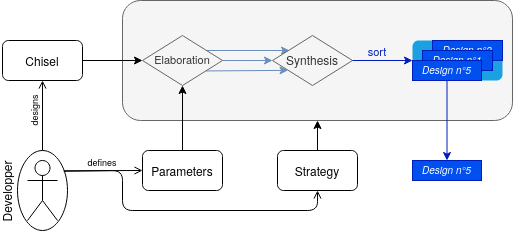
\includegraphics[width=0.85\textwidth]{Figures/DSE-exhaustive}
                \caption{Simple exhaustive strategy\vspace{0.3cm}}
                \label{ch.dse:sec.functional:ssec.complex:fig.complex:sfig.exhaustive}
            \end{subfigure}
            \begin{subfigure}{1.0\textwidth}
                \myAlignmentSpace
                %1.32
                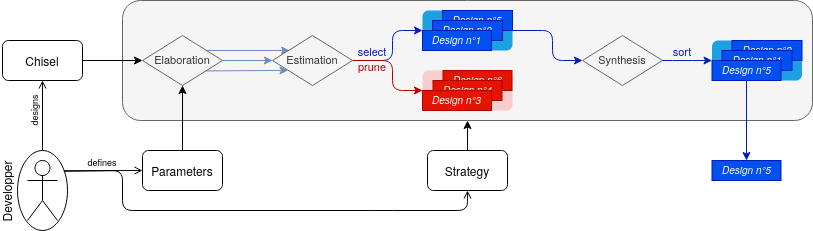
\includegraphics[width=1.36\textwidth]{Figures/DSE-pruning}
                \caption{Pruning based strategy\vspace{0.3cm}}
                \label{ch.dse:sec.functional:ssec.complex:fig.complex:sfig.pruning}
            \end{subfigure}
            \begin{subfigure}{1.0\textwidth}
                \myAlignmentSpace
                %1.19
                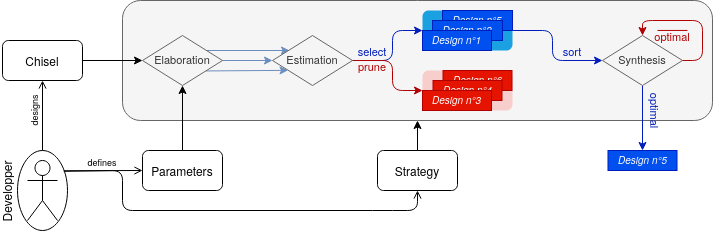
\includegraphics[width=1.23\textwidth]{Figures/DSE-gradient}
                \caption{Gradient descent based strategy}
                \label{ch.dse:sec.functional:ssec.complex:fig.complex:sfig.gradient}
            \end{subfigure}
            \caption{Building complex strategies}
            \label{ch.dse:sec.functional:ssec.complex:fig.complex}
        \end{figure}


%%%%%%%%%%%%%%%%%%%%%%%%%%%%%%%%%%%%%%%%%%%%%%%%%%%%%%%%%%%%%%%%%%%%%%%%%%%%%%%%%

\clearpage
\section[Discussions on the Proposed DSE Methodology]{Discussions on the Proposed Design Space Exploration Methodology}
\label{ch.dse:sec.discussion}
    \subsection{Limitations of the Approach}
    \label{ch.dse:sec.discussion:ssec.limitations}

        Our approach strongly relies on the quality of the estimators to perform quick space traversals while achieving accurate estimations, with the objective to provide realistic solutions.

        It is even more true when looking at the proposed frequency estimation methodology, as it remains as complex as what synthesis is --- in an algorithmic meaning --- and will probably not cope with the \myLongAcs{FPGA}{Field-Programmable Gate Array} specificities, resulting in erroneous estimations after potentially longer processes.
        However, more accurate estimation methods exist at various levels of granularity which could improve the explorations quality, and our methodology would greatly benefit from proposing to its users both multi-level and multi-fidelity estimators \cite{ye_scalehls_2021}\cite{lo_multi-fidelity_2018}.

        On the other hand, more complex exploration schemes are yet to be proposed in order to achieve state of the art exploration performances, notably by using meta heuristics for \myLongAc{MOP}{Multi-objective Optimization Problem} solving (such as \myLongAcs{GA}{Genetic Algorithm} \cite{paletti_dovado_2021}, Bayesian optimization \cite{lo_model-based_2016} or simulated annealing \cite{witschen_circa_2019}), or supervised learning techniques \cite{nardi_practical_2019}\cite{ferretti_leveraging_2020}.

        The proposed schemes are here introduced as a {\it proof of concept} of functional programming usage for efficient \myAc{DSE}, and the introduced library of basic strategies should be enhanced.

    \subsection{Synthesis on the Contributions}
    \label{ch.dse:sec.discussion:ssec.synthesis}

        Using the estimation considerations that were exposed in Chapter \ref{ch.estimators}, as well as the \myLongAcs{HCL}{Hardware Construction Language} features, we defined two complementary methodologies for \myLongAc{DSE}{Design Space Exploration} --- namely {\bf meta design} and {\bf meta exploration}.

        We put a particular focus on how functional programming can be used to define exploration strategies, by leveraging users expertise to build exploration processes step by step.
        We then exposed various basic schemes that can be used to build both application and target specific strategies.

        The proposed methodologies are built considering naive use cases, and both new estimation methodologies and exploration strategies should be proposed in order to provide a more flexible approach.
        

%%%%%%%%%%%%%%%%%%%%%%%%%%%%%%%%%%%%%%%%%%%%%%%%%%%%%%%%%%%%%%%%%%%%%%%%%%%%%%%%%
%%%%%%%%%%%%%%%%%%%%%%%%%%%%%%%%%%%%%%%%%%%%%%%%%%%%%%%%%%%%%%%%%%%%%%%%%%%%%%%
